%  ----------------------------------------------------------------------------
%
%       Copyright (for the thesis) 2009 by [author - insert yourself]
%
%       This thesis is published under the
%       Creative Commons Attribution-No Derivative Works 3.0 Austria License
%       as detailed at http://creativecommons.org/licenses/by-nd/3.0/at/
%
%  ----------------------------------------------------------------------------
%  Template credits and license:
%  ----------------------------------------------------------------------------
%
%       "Fakultät für Informatik" diploma/master thesis template 2008
%
%       based upon "Diploma thesis template 2005" by lukas.silberbauer(at)gmx.at
%       based upon "Diplomarbeit mit LaTeX" by Tobias Erbsland
%       incorporating a title page by Informatik-Forum user "Baby"
%       polished and ported to the TU fonts package by Jakob Petsovits
%
%       published under the terms of
%
%  ----------------------------------------------------------------------------
%  "THE BEER-WARE LICENSE":
%  <lukas.silberbauer(at)gmx.at> wrote this file. As long as you retain this
%  notice you can do whatever you want with this stuff. If we meet some day,
%  and you think this stuff is worth it, you can buy me (us) a beer in return.
%  ----------------------------------------------------------------------------
%
%  (end of template credits)
%

\chapter{Zusätzliche Diagramme}
\label{chap:add_diag}
%\begin{Bild}
%%%%%%%%%%%%%%%%%%%%%%%%%%%%%%%%%%%%%%%%%%%%%%%%%%%%%%%%%%
% Beispieldiagramm mit pgfplot und datenfile
%%%%%%%%%%%%%%%%%%%%%%%%%%%%%%%%%%%%%%%%%%%%%%%%%%%%%%%%%

\begin{tikzpicture}
  \begin{axis}[xlabel=Kameraposition, 
	       ylabel={Zeit (normalisiert)},xtick=\empty]
  \addplot[color=red,
	   mark=|,dashed,
	   only marks,
	   error bars/.cd,
	   y dir=both,
	   y explicit,
	   error bar style={red, error bars options={line width=2pt}}]
    table[col sep=comma,x index=0,y index=2,y error index=3, header=false]
    {data/ReloadTest_Redundance3_R2_D32.2010-1-28.log_medians.data};
  \addlegendentry{Extrema}
  \addplot[color=cyan,
	   mark=|,
	   only marks,
	   error bars/.cd,
	   y dir=both,
	   y explicit,
	   error bar style={cyan, very thick},
	   ultra thick] 
    table[col sep=comma,x index=0,y index=4,y error index=5, header=false]
    {data/ReloadTest_Redundance3_R2_D32.2010-1-28.log_medians.data};
  \addlegendentry{Quartile}
  \addplot[color=black,
	   mark=x,
	   only marks] 
    table[col sep=comma,x index=0,y index=1, header=false]
    {data/ReloadTest_Redundance3_R2_D32.2010-1-28.log_medians.data};
  \addlegendentry{Median}
  \end{axis}
\end{tikzpicture}
%  \captionof{figure}{Reloadtest: Redundanz 3, 2 Renderknoten, 32 Datenknoten.}
%\end{Bild}

%\begin{Bild}
%%%%%%%%%%%%%%%%%%%%%%%%%%%%%%%%%%%%%%%%%%%%%%%%%%%%%%%%%%
% Beispieldiagramm mit pgfplot und datenfile
%%%%%%%%%%%%%%%%%%%%%%%%%%%%%%%%%%%%%%%%%%%%%%%%%%%%%%%%%

\begin{tikzpicture}
  \begin{axis}[xlabel=Kameraposition, 
	       ylabel={Zeit (normalisiert)},xtick=\empty]
  \addplot[color=red,
	   mark=|,dashed,
	   only marks,
	   error bars/.cd,
	   y dir=both,
	   y explicit,
	   error bar style={red, error bars options={line width=2pt}}]
    table[col sep=comma,x index=0,y index=2,y error index=3, header=false]
    {data/ReloadTest_Redundance1_R2_D32.2010-1-27.log_medians.data};
  \addlegendentry{Extrema}
  \addplot[color=cyan,
	   mark=|,
	   only marks,
	   error bars/.cd,
	   y dir=both,
	   y explicit,
	   error bar style={cyan, very thick},
	   ultra thick] 
    table[col sep=comma,x index=0,y index=4,y error index=5, header=false]
    {data/ReloadTest_Redundance1_R2_D32.2010-1-27.log_medians.data};
  \addlegendentry{Quartile}
  \addplot[color=black,
	   mark=x,
	   only marks] 
    table[col sep=comma,x index=0,y index=1, header=false]
    {data/ReloadTest_Redundance1_R2_D32.2010-1-27.log_medians.data};
  \addlegendentry{Median}
  \end{axis}
\end{tikzpicture}
%  \captionof{figure}{Reloadtest: Redundanz 1, 2 Renderknoten, 32 Datenknoten.}
%\end{Bild}

\begin{Bild}
%%%%%%%%%%%%%%%%%%%%%%%%%%%%%%%%%%%%%%%%%%%%%%%%%%%%%%%%%
% Beispieldiagramm mit pgfplot und datenfile
%%%%%%%%%%%%%%%%%%%%%%%%%%%%%%%%%%%%%%%%%%%%%%%%%%%%%%%%%

\begin{tikzpicture}
  \begin{axis}[xlabel=Kameraposition, 
	       ylabel={Zeit (normalisiert)},xtick=\empty]
  \addplot[color=red,
	   mark=|,dashed,
	   only marks,
	   error bars/.cd,
	   y dir=both,
	   y explicit,
	   error bar style={red, error bars options={line width=2pt}}]
    table[col sep=comma,x index=0,y index=2,y error index=3, header=false]
    {data/ReloadTest_Redundance2_R2_D28.2010-1-27.log_medians.data};
  \addlegendentry{Extrema}
  \addplot[color=cyan,
	   mark=|,
	   only marks,
	   error bars/.cd,
	   y dir=both,
	   y explicit,
	   error bar style={cyan, very thick},
	   ultra thick] 
    table[col sep=comma,x index=0,y index=4,y error index=5, header=false]
    {data/ReloadTest_Redundance2_R2_D28.2010-1-27.log_medians.data};
  \addlegendentry{Quartile}
  \addplot[color=black,
	   mark=x,
	   only marks] 
    table[col sep=comma,x index=0,y index=1, header=false]
    {data/ReloadTest_Redundance2_R2_D28.2010-1-27.log_medians.data};
  \addlegendentry{Median}
  \addplot[color=green,
	   no marks] 
    table[col sep=comma,x index=0,y index=6, header=false]
    {data/ReloadTest_Redundance2_R2_D28.2010-1-27.log_medians.data};
  \addlegendentry{Average}
  \end{axis}
\end{tikzpicture}
  \captionof{figure}{Reloadtest: Redundanz 2, 2 Renderknoten, 28 Datenknoten.}
\end{Bild}

\begin{Bild}
%%%%%%%%%%%%%%%%%%%%%%%%%%%%%%%%%%%%%%%%%%%%%%%%%%%%%%%%%
% Beispieldiagramm mit pgfplot und datenfile
%%%%%%%%%%%%%%%%%%%%%%%%%%%%%%%%%%%%%%%%%%%%%%%%%%%%%%%%%

\begin{tikzpicture}
  \begin{axis}[xlabel=Kameraposition, 
	       ylabel={Zeit (in Sekunden)}]
  \addplot+[only marks] 
    table[col sep=comma,x index=0,y index=1, header=false]
    {data/ReloadTest_Redundance3_R2_D24.2010-1-27.log_medians.data};
  \addlegendentry{24 Datenknoten}
  \addplot+[only marks] 
    table[col sep=comma,x index=0,y index=1, header=false]
    {data/ReloadTest_Redundance3_R2_D28.2010-1-28.log_medians.data};
  \addlegendentry{28 Datenknoten}
  \addplot+[only marks] 
    table[col sep=comma,x index=0,y index=1, header=false]
    {data/ReloadTest_Redundance3_R2_D32.2010-1-28.log_medians.data};
  \addlegendentry{32 Datenknoten}
  \end{axis}
\end{tikzpicture}

  \captionof{figure}{Der Median bei 2 Renderern, unterschiedlichen Datenknoten, Redundanz 3 bei unterschiedlichen Kamerapositionen.}
\end{Bild}

\begin{Bild}
%%%%%%%%%%%%%%%%%%%%%%%%%%%%%%%%%%%%%%%%%%%%%%%%%%%%%%%%%
% Beispieldiagramm mit pgfplot und datenfile
%%%%%%%%%%%%%%%%%%%%%%%%%%%%%%%%%%%%%%%%%%%%%%%%%%%%%%%%%

\begin{tikzpicture}
  \begin{axis}[xlabel=Kameraposition, 
	       ylabel={Zeit (in Sekunden)}]
  \addplot+[only marks] 
    table[col sep=comma,x index=0,y index=1, header=false]
    {data/ReloadTest_Redundance1_R2_D32.2010-1-27.log_medians.data};
  \addlegendentry{Redundanz 1}
  \addplot+[only marks] 
    table[col sep=comma,x index=0,y index=1, header=false]
    {data/ReloadTest_Redundance2_R2_D32.2010-1-27.log_medians.data};
  \addlegendentry{Redundanz 2}
  \addplot+[only marks] 
    table[col sep=comma,x index=0,y index=1, header=false]
    {data/ReloadTest_Redundance3_R2_D32.2010-1-28.log_medians.data};
  \addlegendentry{Redundanz 3}
  \end{axis}
\end{tikzpicture}

  \captionof{figure}{Der Median bei 2 Renderern, 32 Datenknoten, unterschiedliche Redundanzen bei unterschiedlichen Kamerapositionen.}
\end{Bild}

\begin{Bild}
%%%%%%%%%%%%%%%%%%%%%%%%%%%%%%%%%%%%%%%%%%%%%%%%%%%%%%%%%
% Beispieldiagramm mit pgfplot und datenfile
%%%%%%%%%%%%%%%%%%%%%%%%%%%%%%%%%%%%%%%%%%%%%%%%%%%%%%%%%

\begin{tikzpicture}
  \begin{axis}[xlabel=Kameraposition, 
	       ylabel={Zeit (in Sekunden)},xtick=\empty]
  \addplot[color=red,
	   mark=|,
	   only marks,
	   error bars/.cd,
	   y dir=both,
	   y explicit,
	   error bar style={red, error bars options={line width=2pt}}]
    table[col sep=comma,x index=0,y index=1,y error index=2, header=false]
    {data/2.data};
  \addlegendentry{Extrema}
  \addplot[color=cyan,
	   mark=|,
	   only marks,
	   error bars/.cd,
	   y dir=both,
	   y explicit,
	   error bar style={cyan, very thick},
	   ultra thick] 
    table[col sep=comma,x index=0,y index=3,y error index=4, header=false]
    {data/2.data};
  \addlegendentry{Quartile}
  \addplot[color=black,
	   mark=x,
	   only marks] 
    table[col sep=comma,x index=0,y index=5, header=false]
    {data/2.data};
  \addlegendentry{Median}
  \end{axis}
\end{tikzpicture}

  \captionof{figure}{Position 2 für 32 Knoten und Redundanz 3 jeweils Extrema, die Quartile und der Median}
\end{Bild}

\begin{Bild}
%%%%%%%%%%%%%%%%%%%%%%%%%%%%%%%%%%%%%%%%%%%%%%%%%%%%%%%%%
% Beispieldiagramm mit pgfplot und datenfile
%%%%%%%%%%%%%%%%%%%%%%%%%%%%%%%%%%%%%%%%%%%%%%%%%%%%%%%%%

\begin{tikzpicture}
  \begin{axis}[xlabel=Kameraposition, 
	       ylabel={Zeit (in Sekunden)}]
  \addplot[color=red,
	   mark=|,
	   only marks,
	   error bars/.cd,
	   y dir=both,
	   y explicit,
	   error bar style={red, error bars options={line width=2pt}}] 
    coordinates { (2,-2.8559703) +- (0.1,1) 
		  (3,-3.5301677) +- (0.1,1) 
		  (4,-4.3050655) +- (0.1,1) 
		  (5,-5.1413136) +- (0.1,1) 
		  (6,-6.0322865) +- (0.1,1) 
		  (7,-6.9675052) +- (0.1,1) 
		  (8,-7.9377747) }; 
  \addplot[color=cyan,
	   mark=|,
	   only marks,
	   error bars/.cd,
	   y dir=both,
	   y explicit,
	   error bar style={cyan, very thick},
	   ultra thick] 
    coordinates { (2,-2.8559703) +- (0.1,0.5) 
		  (3,-3.5301677) +- (0.1,0.5) 
		  (4,-4.3050655) +- (0.1,0.5) 
		  (5,-5.1413136) +- (0.1,0.5) 
		  (6,-6.0322865) +- (0.1,0.5) 
		  (7,-6.9675052) +- (0.1,0.5) 
		  (8,-7.9377747) }; 
  \addplot[color=black,
	   mark=x,
	   only marks] 
    coordinates { (2,-2.8559703) +- (0.1,0.5) 
		  (3,-3.5301677) +- (0.1,0.5) 
		  (4,-4.3050655) +- (0.1,0.5) 
		  (5,-5.1413136) +- (0.1,0.5) 
		  (6,-6.0322865) +- (0.1,0.5) 
		  (7,-6.9675052) +- (0.1,0.5) 
		  (8,-7.9377747) }; 
  \addplot[color=red,
	   mark=|,
	   only marks,
	   error bars/.cd,
	   y dir=both,
	   y explicit,
	   error bar style={red, error bars options={line width=2pt}}] 
    coordinates { (2.5,-2.8559703) +- (0.1,1) 
		  (3.5,-3.5301677) +- (0.1,1) 
		  (4.5,-4.3050655) +- (0.1,1) 
		  (5.5,-5.1413136) +- (0.1,1) 
		  (6.5,-6.0322865) +- (0.1,1) 
		  (7.5,-6.9675052) +- (0.1,1) 
		  (8.5,-7.9377747) }; 
  \addplot[color=cyan,
	   mark=|,
	   only marks,
	   error bars/.cd,
	   y dir=both,
	   y explicit,
	   error bar style={cyan, very thick},
	   ultra thick] 
    coordinates { (2.5,-2.8559703) +- (0.1,0.5) 
		  (3.5,-3.5301677) +- (0.1,0.5) 
		  (4.5,-4.3050655) +- (0.1,0.5) 
		  (5.5,-5.1413136) +- (0.1,0.5) 
		  (6.5,-6.0322865) +- (0.1,0.5) 
		  (7.5,-6.9675052) +- (0.1,0.5) 
		  (8.5,-7.9377747) }; 
  \addplot[color=black,
	   mark=x,
	   only marks] 
    coordinates { (2.5,-2.8559703) +- (0.1,0.5) 
		  (3.5,-3.5301677) +- (0.1,0.5) 
		  (4.5,-4.3050655) +- (0.1,0.5) 
		  (5.5,-5.1413136) +- (0.1,0.5) 
		  (6.5,-6.0322865) +- (0.1,0.5) 
		  (7.5,-6.9675052) +- (0.1,0.5) 
		  (8.5,-7.9377747) }; 
  \end{axis}
\end{tikzpicture}

  \captionof{figure}{TEST}
\end{Bild}

\begin{Bild}
%%%%%%%%%%%%%%%%%%%%%%%%%%%%%%%%%%%%%%%%%%%%%%%%%%%%%%%%%
% Beispieldiagramm mit pgfplot und datenfile
%%%%%%%%%%%%%%%%%%%%%%%%%%%%%%%%%%%%%%%%%%%%%%%%%%%%%%%%%

\begin{tikzpicture}
  \begin{axis}[xlabel=Kameraposition, ylabel={Zeit (in Sekunden)}]
    \addplot table[col sep=comma,x index=0,y index=1,header=false] {data/ReloadTest_Redundance3_R2_D32.2010-1-25.log};
    %\addlegendentry{DataNode0}
    \addplot table[col sep=comma,x index=0,y index=2,header=false] {data/ReloadTest_Redundance3_R2_D32.2010-1-25.log};
    %\addlegendentry{DataNode1}
    \addplot table[col sep=comma,x index=0,y index=3,header=false] {data/ReloadTest_Redundance3_R2_D32.2010-1-25.log};
    %\addlegendentry{DataNode2}
    \addplot table[col sep=comma,x index=0,y index=4,header=false] {data/ReloadTest_Redundance3_R2_D32.2010-1-25.log};
    %\addlegendentry{DataNode3}
    \addplot table[col sep=comma,x index=0,y index=5,header=false] {data/ReloadTest_Redundance3_R2_D32.2010-1-25.log};
    %\addlegendentry{DataNode4}
    \addplot table[col sep=comma,x index=0,y index=6,header=false] {data/ReloadTest_Redundance3_R2_D32.2010-1-25.log};
    %\addlegendentry{DataNode5}
    \addplot table[col sep=comma,x index=0,y index=7,header=false] {data/ReloadTest_Redundance3_R2_D32.2010-1-25.log};
    %\addlegendentry{DataNode6}
    \addplot table[col sep=comma,x index=0,y index=8,header=false] {data/ReloadTest_Redundance3_R2_D32.2010-1-25.log};
    %\addlegendentry{DataNode7}
    \addplot table[col sep=comma,x index=0,y index=9,header=false] {data/ReloadTest_Redundance3_R2_D32.2010-1-25.log};
    %\addlegendentry{DataNode8}
    \addplot table[col sep=comma,x index=0,y index=10,header=false] {data/ReloadTest_Redundance3_R2_D32.2010-1-25.log};
    %\addlegendentry{DataNode9}
    \addplot table[col sep=comma,x index=0,y index=11,header=false] {data/ReloadTest_Redundance3_R2_D32.2010-1-25.log};
    %\addlegendentry{DataNode10}
    \addplot table[col sep=comma,x index=0,y index=12,header=false] {data/ReloadTest_Redundance3_R2_D32.2010-1-25.log};
    %\addlegendentry{DataNode11}
    \addplot table[col sep=comma,x index=0,y index=13,header=false] {data/ReloadTest_Redundance3_R2_D32.2010-1-25.log};
    %\addlegendentry{DataNode12}
    \addplot table[col sep=comma,x index=0,y index=14,header=false] {data/ReloadTest_Redundance3_R2_D32.2010-1-25.log};
    %\addlegendentry{DataNode13}
    \addplot table[col sep=comma,x index=0,y index=15,header=false] {data/ReloadTest_Redundance3_R2_D32.2010-1-25.log};
    %\addlegendentry{DataNode14}
    \addplot table[col sep=comma,x index=0,y index=16,header=false] {data/ReloadTest_Redundance3_R2_D32.2010-1-25.log};
    %\addlegendentry{DataNode15}
    \addplot table[col sep=comma,x index=0,y index=17,header=false] {data/ReloadTest_Redundance3_R2_D32.2010-1-25.log};
    %\addlegendentry{DataNode16}
    \addplot table[col sep=comma,x index=0,y index=18,header=false] {data/ReloadTest_Redundance3_R2_D32.2010-1-25.log};
    %\addlegendentry{DataNode17}
    \addplot table[col sep=comma,x index=0,y index=19,header=false] {data/ReloadTest_Redundance3_R2_D32.2010-1-25.log};
    %\addlegendentry{DataNode18}
    \addplot table[col sep=comma,x index=0,y index=20,header=false] {data/ReloadTest_Redundance3_R2_D32.2010-1-25.log};
    %\addlegendentry{DataNode19}
    \addplot table[col sep=comma,x index=0,y index=21,header=false] {data/ReloadTest_Redundance3_R2_D32.2010-1-25.log};
    %\addlegendentry{DataNode20}
    \addplot table[col sep=comma,x index=0,y index=22,header=false] {data/ReloadTest_Redundance3_R2_D32.2010-1-25.log};
    %\addlegendentry{DataNode21}
    \addplot table[col sep=comma,x index=0,y index=23,header=false] {data/ReloadTest_Redundance3_R2_D32.2010-1-25.log};
    %\addlegendentry{DataNode22}
    \addplot table[col sep=comma,x index=0,y index=24,header=false] {data/ReloadTest_Redundance3_R2_D32.2010-1-25.log};
    %\addlegendentry{DataNode23}
    \addplot table[col sep=comma,x index=0,y index=25,header=false] {data/ReloadTest_Redundance3_R2_D32.2010-1-25.log};
    %\addlegendentry{DataNode24}
    \addplot table[col sep=comma,x index=0,y index=26,header=false] {data/ReloadTest_Redundance3_R2_D32.2010-1-25.log};
    %\addlegendentry{DataNode25}
    \addplot table[col sep=comma,x index=0,y index=27,header=false] {data/ReloadTest_Redundance3_R2_D32.2010-1-25.log};
    %\addlegendentry{DataNode26}
    \addplot table[col sep=comma,x index=0,y index=28,header=false] {data/ReloadTest_Redundance3_R2_D32.2010-1-25.log};
    %\addlegendentry{DataNode27}
    \addplot table[col sep=comma,x index=0,y index=29,header=false] {data/ReloadTest_Redundance3_R2_D32.2010-1-25.log};
    %\addlegendentry{DataNode28}
    \addplot table[col sep=comma,x index=0,y index=30,header=false] {data/ReloadTest_Redundance3_R2_D32.2010-1-25.log};
    %\addlegendentry{DataNode29}
    \addplot table[col sep=comma,x index=0,y index=31,header=false] {data/ReloadTest_Redundance3_R2_D32.2010-1-25.log};
    %\addlegendentry{DataNode30}
    \addplot table[col sep=comma,x index=0,y index=32,header=false] {data/ReloadTest_Redundance3_R2_D32.2010-1-25.log};
    %\addlegendentry{DataNode31}
    \addplot table[col sep=comma,x index=0,y index=33,header=false] {data/ReloadTest_Redundance3_R2_D32.2010-1-25.log};
    %\addlegendentry{Average}
  \end{axis}
\end{tikzpicture}

  \captionof{figure}{\label{fig:eval:reaload1}Zeit zum Vollständigen Neuladen an einer Kameraposition. (Redundanz$=$3, 2 Renderer und 32 Datenknoten)}
\end{Bild}

\begin{Bild}
%%%%%%%%%%%%%%%%%%%%%%%%%%%%%%%%%%%%%%%%%%%%%%%%%%%%%%%%%
% Beispieldiagramm mit pgfplot und datenfile
%%%%%%%%%%%%%%%%%%%%%%%%%%%%%%%%%%%%%%%%%%%%%%%%%%%%%%%%%

\begin{tikzpicture}
  \begin{axis}[xlabel=Kameraposition, ylabel={Zeit (in Sekunden)}]
    \addplot+[only marks] table[col sep=comma,x index=0,y index=1,header=false] {data/ReloadTest_Redundance2_R2_D32.2010-1-26.log};
    %\addlegendentry{DataNode0}
    \addplot+[only marks] table[col sep=comma,x index=0,y index=2,header=false] {data/ReloadTest_Redundance2_R2_D32.2010-1-26.log};
    %\addlegendentry{DataNode1}
    \addplot+[only marks] table[col sep=comma,x index=0,y index=3,header=false] {data/ReloadTest_Redundance2_R2_D32.2010-1-26.log};
    %\addlegendentry{DataNode2}
    \addplot+[only marks] table[col sep=comma,x index=0,y index=4,header=false] {data/ReloadTest_Redundance2_R2_D32.2010-1-26.log};
    %\addlegendentry{DataNode3}
    \addplot+[only marks] table[col sep=comma,x index=0,y index=5,header=false] {data/ReloadTest_Redundance2_R2_D32.2010-1-26.log};
    %\addlegendentry{DataNode4}
    \addplot+[only marks] table[col sep=comma,x index=0,y index=6,header=false] {data/ReloadTest_Redundance2_R2_D32.2010-1-26.log};
    %\addlegendentry{DataNode5}
    \addplot+[only marks] table[col sep=comma,x index=0,y index=7,header=false] {data/ReloadTest_Redundance2_R2_D32.2010-1-26.log};
    %\addlegendentry{DataNode6}
    \addplot+[only marks] table[col sep=comma,x index=0,y index=8,header=false] {data/ReloadTest_Redundance2_R2_D32.2010-1-26.log};
    %\addlegendentry{DataNode7}
    \addplot+[only marks] table[col sep=comma,x index=0,y index=9,header=false] {data/ReloadTest_Redundance2_R2_D32.2010-1-26.log};
    %\addlegendentry{DataNode8}
    \addplot+[only marks] table[col sep=comma,x index=0,y index=10,header=false] {data/ReloadTest_Redundance2_R2_D32.2010-1-26.log};
    %\addlegendentry{DataNode9}
    \addplot+[only marks] table[col sep=comma,x index=0,y index=11,header=false] {data/ReloadTest_Redundance2_R2_D32.2010-1-26.log};
    %\addlegendentry{DataNode10}
    \addplot+[only marks] table[col sep=comma,x index=0,y index=12,header=false] {data/ReloadTest_Redundance2_R2_D32.2010-1-26.log};
    %\addlegendentry{DataNode11}
    \addplot+[only marks] table[col sep=comma,x index=0,y index=13,header=false] {data/ReloadTest_Redundance2_R2_D32.2010-1-26.log};
    %\addlegendentry{DataNode12}
    \addplot+[only marks] table[col sep=comma,x index=0,y index=14,header=false] {data/ReloadTest_Redundance2_R2_D32.2010-1-26.log};
    %\addlegendentry{DataNode13}
    \addplot+[only marks] table[col sep=comma,x index=0,y index=15,header=false] {data/ReloadTest_Redundance2_R2_D32.2010-1-26.log};
    %\addlegendentry{DataNode14}
    \addplot+[only marks] table[col sep=comma,x index=0,y index=16,header=false] {data/ReloadTest_Redundance2_R2_D32.2010-1-26.log};
    %\addlegendentry{DataNode15}
    \addplot+[only marks] table[col sep=comma,x index=0,y index=17,header=false] {data/ReloadTest_Redundance2_R2_D32.2010-1-26.log};
    %\addlegendentry{DataNode16}
    \addplot+[only marks] table[col sep=comma,x index=0,y index=18,header=false] {data/ReloadTest_Redundance2_R2_D32.2010-1-26.log};
    %\addlegendentry{DataNode17}
    \addplot+[only marks] table[col sep=comma,x index=0,y index=19,header=false] {data/ReloadTest_Redundance2_R2_D32.2010-1-26.log};
    %\addlegendentry{DataNode18}
    \addplot+[only marks] table[col sep=comma,x index=0,y index=20,header=false] {data/ReloadTest_Redundance2_R2_D32.2010-1-26.log};
    %\addlegendentry{DataNode19}
    \addplot+[only marks] table[col sep=comma,x index=0,y index=21,header=false] {data/ReloadTest_Redundance2_R2_D32.2010-1-26.log};
    %\addlegendentry{DataNode20}
    \addplot+[only marks] table[col sep=comma,x index=0,y index=22,header=false] {data/ReloadTest_Redundance2_R2_D32.2010-1-26.log};
    %\addlegendentry{DataNode21}
    \addplot+[only marks] table[col sep=comma,x index=0,y index=23,header=false] {data/ReloadTest_Redundance2_R2_D32.2010-1-26.log};
    %\addlegendentry{DataNode22}
    \addplot+[only marks] table[col sep=comma,x index=0,y index=24,header=false] {data/ReloadTest_Redundance2_R2_D32.2010-1-26.log};
    %\addlegendentry{DataNode23}
    \addplot+[only marks] table[col sep=comma,x index=0,y index=25,header=false] {data/ReloadTest_Redundance2_R2_D32.2010-1-26.log};
    %\addlegendentry{DataNode24}
    \addplot+[only marks] table[col sep=comma,x index=0,y index=26,header=false] {data/ReloadTest_Redundance2_R2_D32.2010-1-26.log};
    %\addlegendentry{DataNode25}
    \addplot+[only marks] table[col sep=comma,x index=0,y index=27,header=false] {data/ReloadTest_Redundance2_R2_D32.2010-1-26.log};
    %\addlegendentry{DataNode26}
    \addplot+[only marks] table[col sep=comma,x index=0,y index=28,header=false] {data/ReloadTest_Redundance2_R2_D32.2010-1-26.log};
    %\addlegendentry{DataNode27}
    \addplot+[only marks] table[col sep=comma,x index=0,y index=29,header=false] {data/ReloadTest_Redundance2_R2_D32.2010-1-26.log};
    %\addlegendentry{DataNode28}
    \addplot+[only marks] table[col sep=comma,x index=0,y index=30,header=false] {data/ReloadTest_Redundance2_R2_D32.2010-1-26.log};
    %\addlegendentry{DataNode29}
    \addplot+[only marks] table[col sep=comma,x index=0,y index=31,header=false] {data/ReloadTest_Redundance2_R2_D32.2010-1-26.log};
    %\addlegendentry{DataNode30}
    \addplot+[only marks] table[col sep=comma,x index=0,y index=32,header=false] {data/ReloadTest_Redundance2_R2_D32.2010-1-26.log};
    %\addlegendentry{DataNode31}
    \addplot+[only marks] table[col sep=comma,x index=0,y index=33,header=false] {data/ReloadTest_Redundance2_R2_D32.2010-1-26.log};
    %\addlegendentry{Average}
  \end{axis}
\end{tikzpicture}

  \captionof{figure}{\label{fig:eval:reload2}Zeit zum Vollständigen Neuladen an einer Kameraposition. (Redundanz$=$2, 2 Renderer und 32 Datenknoten)}
\end{Bild}

\begin{Bild}
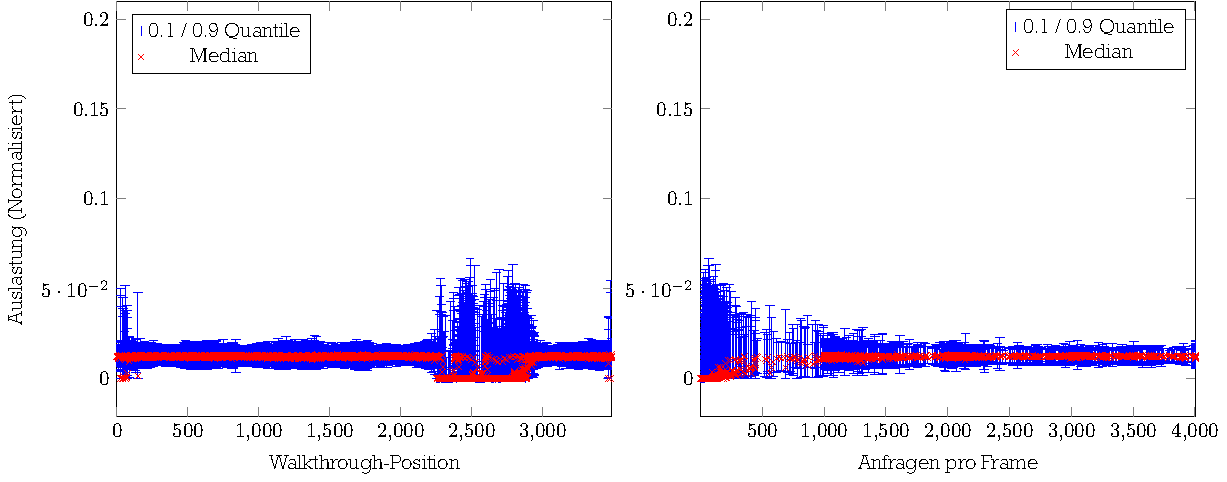
\includegraphics[scale=0.75]{images/diag_cCol_red1_render4_data80_2x.pdf}
  \captionof{figure}{\label{fig:eval:cCol2}Die Auslastung der Datenknoten in einem Walkthrough bei 4 Renderknoten und 80 Datenknoten und Redundanz$=$1.}
\end{Bild}

\begin{Bild}
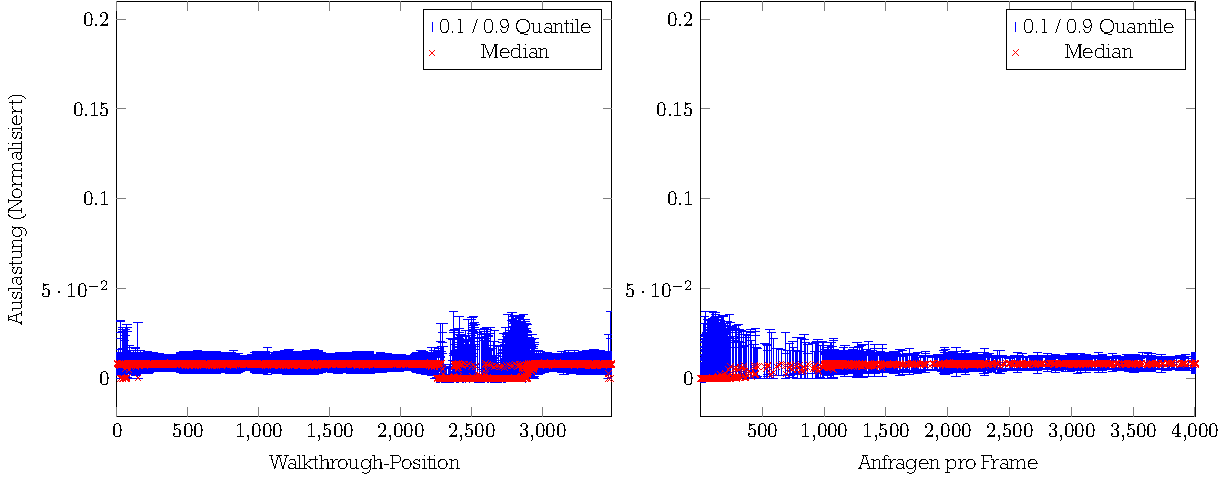
\includegraphics[scale=0.75]{images/diag_cCol_red1_render4_data120_2x.pdf}
  \captionof{figure}{\label{fig:eval:cCol3}Die Auslastung der Datenknoten in einem Walkthrough bei 4 Renderknoten und 120 Datenknoten und Redundanz$=$1.}
\end{Bild}

\begin{Bild}
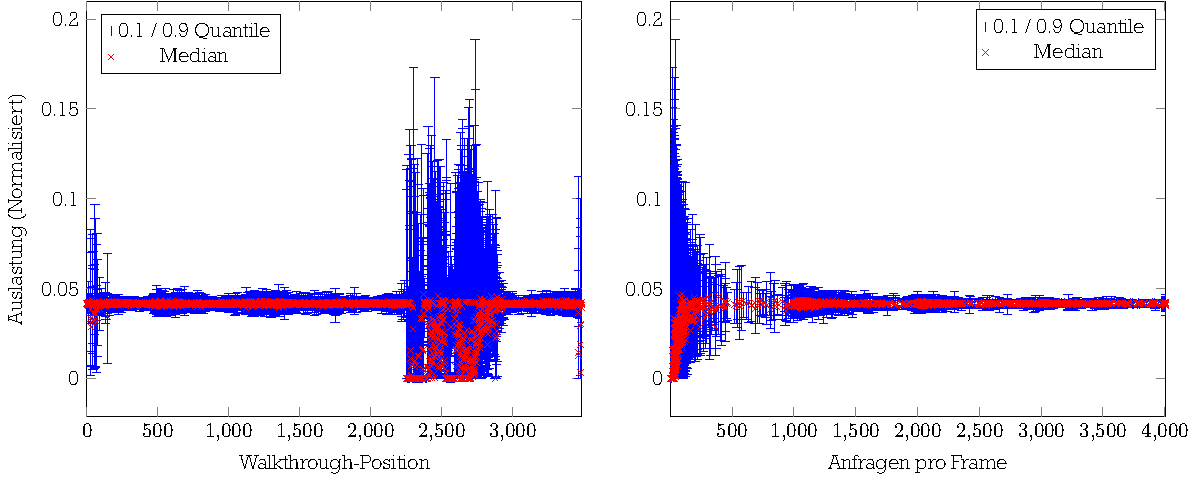
\includegraphics[scale=0.75]{images/diag_cCol_red2_render4_data24_2x.pdf}
  \captionof{figure}{\label{fig:eval:cCol4}Die Auslastung der Datenknoten in einem Walkthrough bei 4 Renderknoten und 24 Datenknoten und Redundanz$=$2.}
\end{Bild}

\begin{Bild}
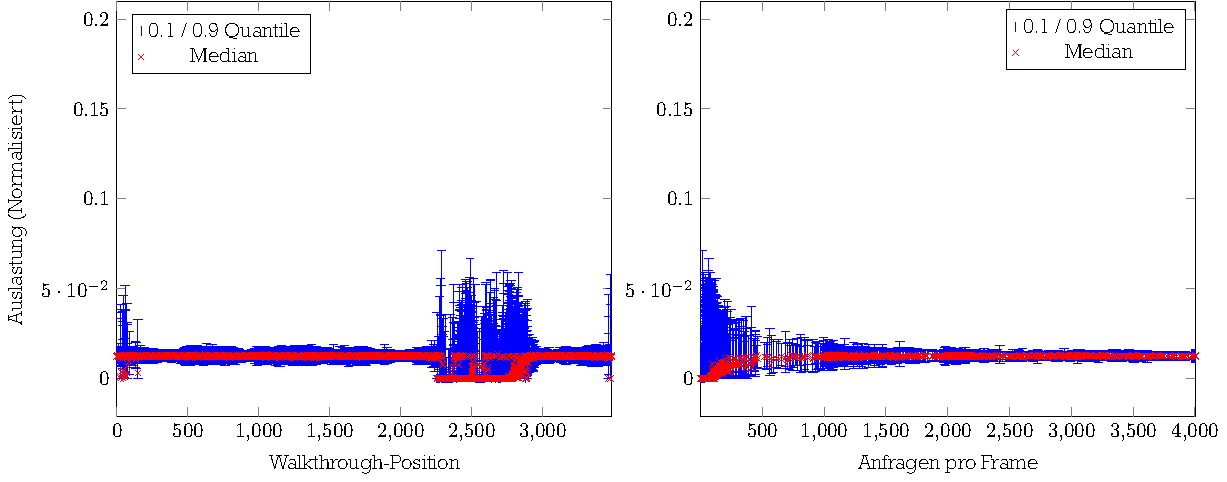
\includegraphics[scale=0.75]{images/diag_cCol_red2_render4_data80_2x.pdf}
  \captionof{figure}{\label{fig:eval:cCol5}Die Auslastung der Datenknoten in einem Walkthrough bei 4 Renderknoten und 80 Datenknoten und Redundanz$=$2.}
\end{Bild}

\begin{Bild}
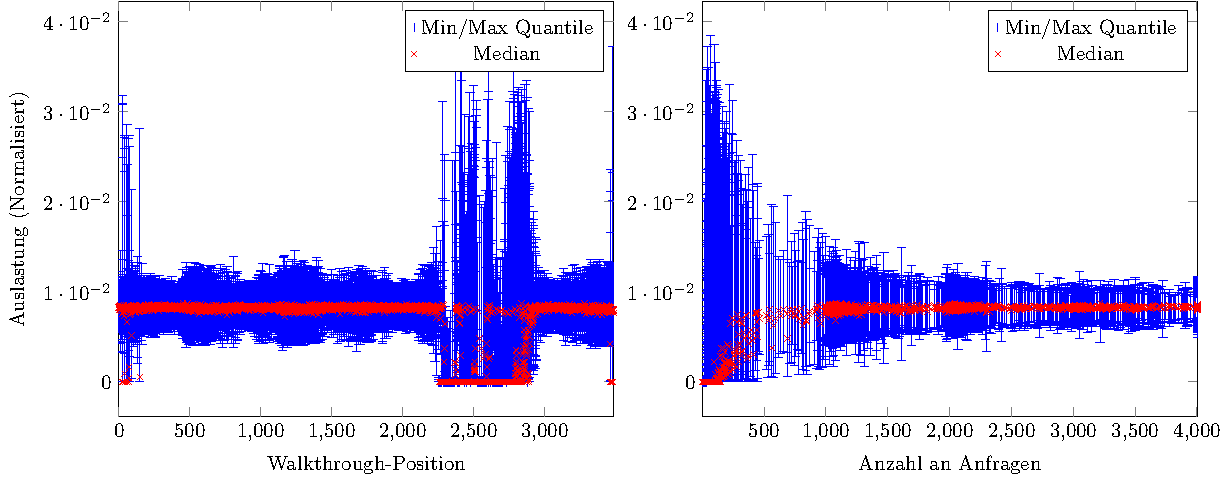
\includegraphics[scale=0.75]{images/diag_cCol_red2_render4_data120_2x.pdf}
  \captionof{figure}{\label{fig:eval:cCol6}Die Auslastung der Datenknoten in einem Walkthrough bei 4 Renderknoten und 120 Datenknoten und Redundanz$=$2.}
\end{Bild}

\begin{Bild}
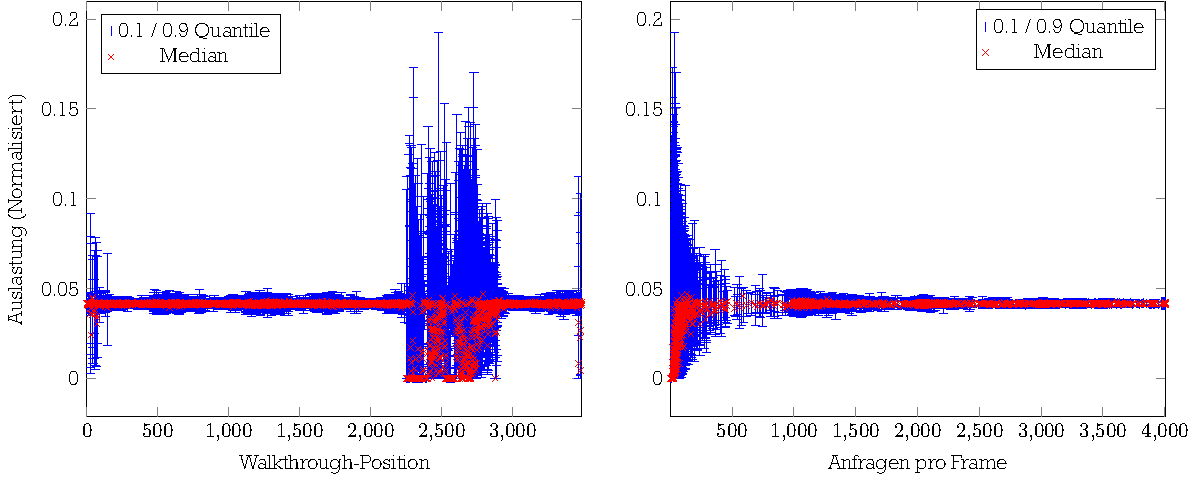
\includegraphics[scale=0.75]{images/diag_cCol_red3_render4_data24_2x.pdf}
  \captionof{figure}{\label{fig:eval:cCol7}Die Auslastung der Datenknoten in einem Walkthrough bei 4 Renderknoten und 24 Datenknoten und Redundanz$=$3.}
\end{Bild}

\begin{Bild}
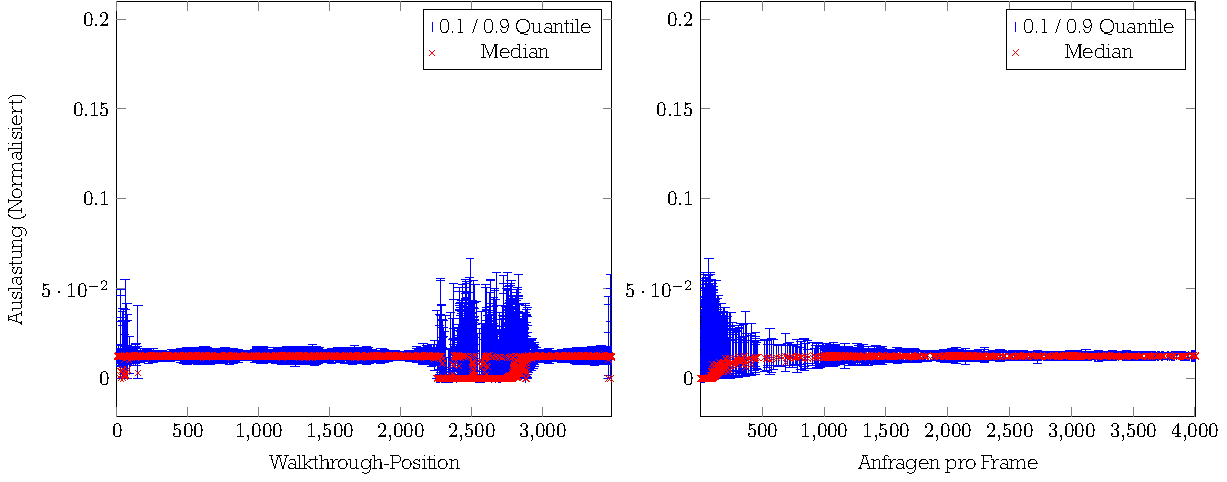
\includegraphics[scale=0.75]{images/diag_cCol_red3_render4_data80_2x.pdf}
  \captionof{figure}{\label{fig:eval:cCol8}Die Auslastung der Datenknoten in einem Walkthrough bei 4 Renderknoten und 80 Datenknoten und Redundanz$=$3.}
\end{Bild}

\begin{Bild}
%%%%%%%%%%%%%%%%%%%%%%%%%%%%%%%%%%%%%%%%%%%%%%%%%%%%%%%%%
% Beispieldiagramm mit pgfplot und datenfile
%%%%%%%%%%%%%%%%%%%%%%%%%%%%%%%%%%%%%%%%%%%%%%%%%%%%%%%%%

\begin{tikzpicture}
  \begin{axis}[xlabel=Position, ylabel={FPS}, ymax=60, legend pos=north west]
    \addplot[smooth,red,samples=500] table[col sep=comma,x index=0,y index=1,header=false] {data/FPSWalkthroughTest_Redundance1_R2_D24.2010-1-25.log};
    \addlegendentry{24 Datenknoten}
    \addplot[smooth,green,samples=500] table[col sep=comma,x index=0,y index=1,header=false] {data/FPSWalkthroughTest_Redundance1_R2_D28.2010-1-25.log};
    \addlegendentry{28 Datenknoten}
    \addplot[smooth,blue,samples=500] table[col sep=comma,x index=0,y index=1,header=false] {data/FPSWalkthroughTest_Redundance1_R2_D32.2010-1-25.log};
    \addlegendentry{32 Datenknoten}
  \end{axis}
\end{tikzpicture}

  \captionof{figure}{\label{fig:eval:fps1}FPS in einem Walkthrough. (Redundanz$=$1, 2 Renderer und 24-32 Datenknoten)}
\end{Bild}

\begin{Bild}
%%%%%%%%%%%%%%%%%%%%%%%%%%%%%%%%%%%%%%%%%%%%%%%%%%%%%%%%%
% Beispieldiagramm mit pgfplot und datenfile
%%%%%%%%%%%%%%%%%%%%%%%%%%%%%%%%%%%%%%%%%%%%%%%%%%%%%%%%%

\begin{tikzpicture}
  \begin{axis}[xlabel=Position, ylabel={FPS}, ymax=60, legend pos=north west]
    \addplot[smooth,red,samples=500] table[col sep=comma,x index=0,y index=1,header=false] {data/FPSWalkthroughTest_Redundance3_R2_D24.2010-1-25.log};
    \addlegendentry{24 Datenknoten}
    \addplot[smooth,green,samples=500] table[col sep=comma,x index=0,y index=1,header=false] {data/FPSWalkthroughTest_Redundance3_R2_D28.2010-1-25.log};
    \addlegendentry{28 Datenknoten}
    \addplot[smooth,blue,samples=500] table[col sep=comma,x index=0,y index=1,header=false] {data/FPSWalkthroughTest_Redundance3_R2_D32.2010-1-25.log};
    \addlegendentry{32 Datenknoten}
  \end{axis}
\end{tikzpicture}

  \captionof{figure}{\label{fig:eval:fps3}FPS in einem Walkthrough. (Redundanz$=$3, 2 Renderer und 24-32 Datenknoten)}
\end{Bild}

%
% EOF
%
